% Für Seitenformatierung

\documentclass[DIV=15]{scrartcl}

% Zeilenumbrüche

\parindent 0pt
\parskip 6pt

% Für deutsche Buchstaben und Synthax

\usepackage[ngerman]{babel}

% Für Auflistung mit speziellen Aufzählungszeichen

\usepackage{paralist}

% zB für \del, \dif und andere Mathebefehle

\usepackage{amsmath}
\usepackage{commath}
\usepackage{amssymb}

% Für Literatur/bibliography

%\usepackage[backend=biber , style=alphabetic , hyperref=true]{biblatex}

% Für \SIunit[]{} und \num in deutschem Stil

\usepackage[output-decimal-marker={,}]{siunitx}
\DeclareSIUnit\clight{\ensuremath{c}}

% Schriftart und encoding

\usepackage[utf8]{inputenc}
% Bitstream charter als default
\usepackage[charter, greekuppercase=italicized]{mathdesign}
% Lato, als sans default
\renewcommand{\sfdefault}{fla}

% Für \sfrac{}{}, also inline-frac

\usepackage{xfrac}

% Für Einbinden von pdf-Grafiken

\usepackage{graphicx}

% Umfließen von Bildern

\usepackage{floatflt}

% Für weitere Farben

\usepackage{color}

% Für Streichen von z.B. $\rightarrow$

\usepackage{centernot}

% Für Befehl \cancel{}

\usepackage{cancel}

% Für Links nach außen und innerhalb des Dokumentes

\usepackage{hyperref}

% Für Layout von Links

\hypersetup{
	citecolor=black,
	colorlinks=true,
	linkcolor=black,
	urlcolor=blue,
}

% Verschiedene Mathematik-Hilfen

\newcommand \e[1]{\cdot10^{#1}}
\newcommand\p{\partial}

\newcommand\half{\frac 12}
\newcommand\shalf{\sfrac12}

\newcommand\skp[2]{\left\langle#1,#2\right\rangle}
\newcommand\mw[1]{\left\langle#1\right\rangle}
\newcommand \eexp[1]{\mathrm{e}^{#1}}
\newcommand \dexp[1]{\exp\del{#1}}
\newcommand \dsin[1]{\sin\del{#1}}
\newcommand \dcos[1]{\cos\del{#1}}
\newcommand \dtan[1]{\tan\del{#1}}
\newcommand \darccos[1]{\arcos\del{#1}}
\newcommand \darcsin[1]{\arcsin\del{#1}}
\newcommand \darctan[1]{\arctan\del{#1}}

% Nabla und Kombinationen von Nabla

\renewcommand\div[1]{\skp{\nabla}{#1}}
\newcommand\rot{\nabla\times}
\newcommand\grad[1]{\nabla#1}
\newcommand\laplace{\triangle}
\newcommand\dalambert{\mathop{{}\Box}\nolimits}

%Für komplexe Zahlen

\newcommand \ii{\mathrm i}
\renewcommand{\Im}{\mathop{{}\mathrm{Im}}\nolimits}
\renewcommand{\Re}{\mathop{{}\mathrm{Re}}\nolimits}

%Für Bra-Ket-Notation

\newcommand\bra[1]{\left\langle#1\right|}
\newcommand\ket[1]{\left|#1\right\rangle}
\newcommand\braket[2]{\left\langle#1\left.\vphantom{#1 #2}\right|#2\right\rangle}
\newcommand\braopket[3]{\left\langle#1\left.\vphantom{#1 #2 #3}\right|#2\left.\vphantom{#1 #2 #3}\right|#3\right\rangle}


\newcounter{thezettel}
\setcounter{thezettel}{3}
\renewcommand\thesection{\arabic{thezettel}.\arabic{section}}


\title{physik421 - Übung \arabic{thezettel}}
\author{Lino Lemmer \\ \small{l2@uni-bonn.de} \and Frederike Schrödel \and Simon Schlepphorst\\ \small{s2@uni-bonn.de}}

\begin{document}
\maketitle

\section{Fouriertransformation}

\subsection{Abbildung von Ableitungsoperator auf Multiplikation}
\begin{align*}
 \mathcal{F}\cbr{\phi}\del{\vec k} &= \frac{1}{\del{2\pi}^{\frac{n}2}} \int^\infty_{-\infty} \dif^{\,n} x \phi\del{\vec x}\ee^{-\ii \vec k \vec x}\\
 \mathcal{F}\cbr{\dpd{}{x_\alpha} f\del x}\del{\vec k} &= \frac1{\del{2\pi}^{\frac{n}{2}}} \int_{-\infty}^\infty \dif^{\,n} x \underbrace{\dpd{}{x_\alpha} f\del{\vec x}}_{u'}
 \underbrace{\ee^{-\ii \vec k \vec x}}_{v}\\
 &= \frac1{\del{2\pi}^{\frac{n}2}} \del{ \sbr{f\del{\vec x}\ee^{-\ii\vec k\vec x}}^\infty_{-\infty}
 + \int_{-\infty}^{\infty} \dif^{\,n} x f\del{\vec x}\del{\ii k_\alpha}\ee^{-\ii \vec k \vec x}}
 \intertext{Damit $f\del{\vec x}$ quadratintegrabel ist, muss $f\del{\pm \infty} \to 0$ gehen}
 \implies &\underbrace{\ii k}_{\dpd{}{x_\alpha}} \mathcal{F}\cbr{f\del{\vec x}}\del{\vec k}\\
 \implies &\mathcal{F}\cbr{\dpd{}{x_\alpha}}\del{\vec k} = \ii k_\alpha\\
 \intertext{Herleitung für $\mathcal{F}\cbr{\dpd{}{k_\alpha}}\del{\vec x}$ funktioniert analog. Nur mit $\ldots \int_{-\infty}^\infty \ldots \ee^{+\ii \vec k \vec x}$}
 \implies &\mathcal{F}\cbr{\dpd{}{k_\alpha}}\del{\vec x} = - \ii k_\alpha
\end{align*}


\subsection{}
\begin{align*}
 \mathcal{F}\cbr{\phi}\del{k} &= \underbrace{\frac1{\sqrt{2\pi}}}_{a} \int_{-\infty}{\infty} \dif t \phi\del{t} \ee^{-\ii \omega t}\\
  &= a \int_{-\infty}^\infty \dif t \del{\phi_e\del{t} + \phi_o\del{t}} \cos\del{\omega t}
  - \ii a \int_{-\infty}^\infty \dif t \del{\phi_e\del{t} + \phi_o\del{t}} \sin\del{\omega t}
  \intertext{mit $\phi\del{t} = \phi_e\del{t} + \phi_o\del{t}$ und $\ee^{-\ii x} = \cos\del{x} - \ii \sin \del{x}$}
\end{align*}
Für Integrale über gerade bzw. ungerade Funktionen gilt:
\begin{align*}
 &\int_{-\infty}^\infty \underbrace{f\del{x}}_{\text{odd}} \underbrace{g\del x}_{\text{even}} = 0
 \quad \quad \text{mit}
 \begin{cases}
  \cos\del x : \text{even} & \cos\del x = \cos\del{-x}\\
  \sin\del x: \text{odd} & \sin\del x = - \sin\del{-x}
 \end{cases}\\
 \implies &\underbrace{a \int_{-\infty}^\infty \dif t \phi_e\del t \cos \del{\omega t}}_{\Re \del{\phi\del t}}
 \underbrace{- \ii a \int_{-\infty}^\infty \dif t \phi_o\del t \sin\del{\omega t}}_{- \ii \Im\del{\phi\del t}}
\end{align*}


\subsection{Abbildung von Produkt auf Faltung}
Für eine Faltung gilt:
\[
  (\phi_1 * \phi_2)(x) =  \int^\infty_{-\infty}\dif^n y \phi_1(x-y)\phi_2(y)
\]

Und für $n=1$ ergibt sich somit:
\begin{align}
  \sqrt{2\pi} \mathcal{F}\{\phi_1 \cdot \phi_2\} (k) &= \int^\infty_{-\infty}\dif x \phi_1(x)\phi_2(x) \ee^{-ikx}	\\
  &= \int^\infty_{-\infty}\dif x \int^\infty_{-\infty}\dif y \phi_1(x-y)\phi_2(y) \ee^{-ik(x-y)} \ee^{-iky}	\\
  &= \left(\mathcal{F}\{\phi_1\}*\mathcal{F}\{\phi_1\}\right) (k)
\end{align}


\subsection{Vertauschbarkeit von Ableitung und Faltung}
Da die Ableitung unabhängig von den Variablen des Integrals ist, lässt sie sich in das Integral ziehen:
\begin{align}
  \frac{\partial}{\partial x_\alpha} \left((\phi_1 * \phi_2)(x)\right) &= \frac{\partial}{\partial x_\alpha} \left(\int^\infty_{-\infty}\dif^n y \phi_1(x-y)\phi_2(y)\right)	\\
  &= \int^\infty_{-\infty}\dif^n y \left(\frac{\partial}{\partial x_\alpha} \phi_1(x-y)\right)\phi_2(y)	\\
  &= \left(\partial_\alpha \phi_1 * \phi_2\right)(x)
\end{align}


\section{Gaußintegrale}
Für diese Aufgabe ist eine Wahrscheinlichkeitsdichte von 
\[
    p(x) = C\ee^{-\frac 12ax^2=bx} 
\]
wobei $x$ eine Zufallsgröße ist und gilt: $a,b\in\Re$ und $a>0$.

\subsection{Identität}
Es soll gezeigt werden, dass gilt:
\[
    I = \int^\infty_{-\infty}\ee^{\frac{x^2}{2}}\dif x = \sqrt{2\pi}
\]
Den Tipp nutzend berechne ich zunächst $I^2$ und schreib dies dann mit $\vec x = r(\cos\phi,\sin\phi)$ und $\dif^2x = r\dif r\dif\phi$  in Polarkoordinaten um.
\begin{align*}
    I^2 &= \int^\infty_{-\infty}\dif x\ee^{-\frac{x^2}{2}}\int^\infty_{-\infty}\dif y\ee^{-\frac{y^2}{2}} \\
        &= \int_{\Re^2}\dif^2x\ee^{\frac{x^2}{2}} \\
        &= \int^{2\pi}_0\dif\phi\int^\infty_0\dif rr\ee^{-\frac{r^2}{2}} \\
\end{align*}
an dieser Stelle nutze ich folgenden Trick:
\begin{align*}
    \dod {\ee^{-\frac{r^2}{2}}}{r} &= \frac{-r}{2}\ee^{\frac{-r^2}{2}} \\
    \implies \int -\frac r2 \ee^{\frac{r^2}2} &= \ee^{\frac{r^2}2} \\
    \implies -2\int -\frac r2 \ee^{\frac{r^2}2} &= -2\ee^{\frac{r^2}2} \\
\end{align*}
Wenn ich damit weiter rechne erhalte ich als gesammt Lösung des Integrals:
\begin{align*}
    I^2 &= \int^{2\pi}_0\dif\phi\int^\infty_0\dif rr\ee^{-\frac{r^2}{2}} \\
        &=-2\pi\ee^{-\frac{r^2}2}|^\infty_{r=0} \\
        &= 2\pi \\
    I &= \sqrt{2\pi}
\end{align*}
Somit haben wir es gezeigt.

\subsection{Normierung}
Nach einer Normierung muss das Integral der Wahrscheinlcihkeitsdichte über den Raum eins ergeben.
\begin{align*}
    \int^\infty_{-\infty} P(x)\dif x &= int^\infty_{-\infty}\dif xC\ee^{-\frac 12ax^2+bx} \\
                                     &= 1 \\
\end{align*}
Zunächst formen wir den Exponenten um und substituieren.
\begin{align*}
    -\frac 12a^2+bx &= -\frac 12a(x^2-2\frac bax) \\
                    &= -\frac 12a(x^2-2\frac bax+\frac{b^2}{a^2}-\frac{b^2}{a^2}) \\
                    &= -\frac 12a[(x-\frac ba)^2-\frac{b^2}{a^2}] \\
\end{align*}
Mit $\xi := x-\frac ba$ erhalten wir $\ee^{1\frac 12 a(\xi^2-\frac{b^2}{a^2})}$.
Nun kann man über di Potenzgesetze die $\ee$-Funktion auseinander ziehen und den konstanten Term mit dem $C$ vor das Integral Ziehen.
\begin{align*}
    1&:= C\ee^{\frac{b^2}{2a}}\int^\infty_{-\infty}\dif\xi\ee^{-\frac 12a\xi^2} \qquad|\text{ mit }\psi^2 = \frac 12a\xi^2 \implies \psi=\sqrt{\frac a2}\xi \implies \dif\xi=\sqrt{\frac 2a}\dif \psi\\ 
     &= C\ee^{\frac{b^2}{2a}}\sqrt{\frac 2a}\int^\infty_{-\infty}\dif\psi\ee^{-\psi^2} \\
     &= C\ee^{\frac{b^2}{2a}}\sqrt{\frac 2a}\sqrt{\pi} \\
     \implies C &= \frac{1}{\ee^{\frac{b^2}{2a}}\sqrt{\frac 2a}\sqrt{\pi}} \\
\end{align*}

\subsection{Mittelwert}
Da es sich offensichtlich um eine Gaußverteilung handelt ist der Mittelwert gegeben durch den Mittelpunkt der Gaußverteilung.


\section{Freies Wellenpaket}
Gegeben ist ein eindimensionales Wellenpacket $\psi\del{x,0}$ durch seine Fouriertransformierte
\begin{align*}
	\phi\del{k,0}=A\ee^{\del{k-k_0}^2d^2}, &&\text{mit }k_0,A\text{ und }d>0
\end{align*}
und die, wiederum durch Fouriertransformation, rücktransformierte Wellengleichung
\begin{align*}
	\psi\del{x,t}=\frac{A}{\sqrt{2}\pi}\int_{-\infty}^{\infty}\dif k\;\ee^{-\del{k-k_0}^2d^2-\ii\frac{\hbar^2k^2}{2m}t+\ii kx}
\end{align*}

\subsection{Impulsverteilung}
% \subsection{Skizze im Impulsraum}
Nun soll zuerst das im Impulsraum gegebene Wellenpacket $\phi\del{k,0}$ skizziert werden. Dies habe ich, unter Verwendung von GNU-Plot, für verschiedene $k_0$, $d$ und $A$, in Abbildung 1 realisiert. Diese zeigt, dass $A$ die Position des Maximums, $d$ die Breite und $k_0$ die Position des Wellenpackets festlegen. Dabei wurde natürlich vernachlässigt, dass $A$ noch nicht genormt worden ist.
\begin{figure}[ht]
	\centering
	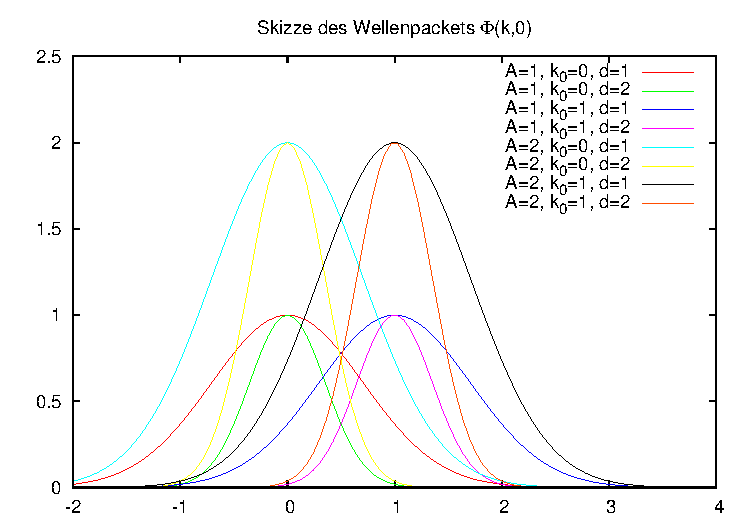
\includegraphics[scale=1.3]{Skizze_zu_3_1.pdf}
	\caption{Wellenpacket $\phi\del{k,0}$ im Impulsraum für verschiedene $k_0$, $d$ und $A$}
\end{figure}

\subsection{Wahrscheinlichkeitsdichte}
% \subsection{Ausführen der Fouriertransformation und Dichte}
Ich führe nun obiges Integral aus:
\begin{align*}
	\psi\del{x,t}&=\frac{A}{\sqrt{2}\pi}\int_{-\infty}^{\infty}\dif k\;\ee^{-\del{k-k_0}^2d^2-\ii\frac{\hbar^2k^2}{2m}t+\ii kx}\\
	&=\frac{A}{\sqrt{2}\pi}\int_{-\infty}^{\infty}\dif k\;\ee^{-k^2d^2+2kk_0d^2-k_0^2d^2-\ii\frac{\hbar^2k^2}{2m}t+\ii kx}\\
	&=\frac{A}{\sqrt{2}\pi}\ee^{-k_0^2d^2}\int_{-\infty}^{\infty}\dif k\;\ee^{-k^2\del{d^2+\ii\frac{\hbar^2}{2m}t}+k\del{2k_0d^2+\ii x}}\\
	\intertext{
		setze
		\[
			\alpha\equiv\alpha\del{t}=\del{d^2+\ii\frac{\hbar^2}{2m}t}\text{ und }2\beta\equiv2\beta\del{x}=\del{2k_0d^2+\ii x}
		\]
	}
	&=\frac{A}{\sqrt{2}\pi}\ee^{-k_0^2d^2}\int_{-\infty}^{\infty}\dif k\;\ee^{-\alpha\del{k^2-2\beta k+\beta^2-\beta^2}}\\
	&=\frac{A}{\sqrt{2}\pi}\ee^{\alpha\beta^2-k_0^2d^2}
	\underbrace{\int_{-\infty}^{\infty}\dif k\;\ee^{-\alpha\del{k-\beta}^2}}_{=\frac{\sqrt{\pi}}{\sqrt{\alpha}}}\\
	&=\frac{A}{\sqrt{2\pi\alpha}}\ee^{\alpha\beta^2-k_0^2d^2}\\
	&=\frac{A}{\sqrt{2\pi\del{d^2+\ii\frac{\hbar^2}{2m}t}}}\ee^{\frac14\del{d^2+\ii\frac{\hbar^2}{2m}t}\del{2k_0d^2+\ii x}^2-k_0^2d^2}
\end{align*}
Mit diesem Ergebnis soll nun die Dichte der Aufenthaltswahrscheinlichkeit berechnet werden:
\begin{align*}
	\abs{\psi\del{x,t}}^2&=\psi\del{x,t}\psi^*\del{x,t}\\
	&=\frac{A}{\sqrt{2\pi\alpha}}\ee^{\alpha\beta^2-k_0^2d^2}\frac{A}{\sqrt{2\pi\alpha^*}}\ee^{\alpha^*{\beta^*}^2-k_0^2d^2}\\
	&=\frac{A^2}{2\pi\sqrt{\alpha\alpha^*}}\ee^{\alpha\beta^2+\alpha^*{\beta^*}^2-2k_0^2d^2}\\
	&=\frac{A^2}{2\pi\abs{\alpha}}\ee^{2\Re\del{\alpha\beta^2}-2k_0^2d^2}\\
	&=\frac{A^2}{2\pi\sqrt{d^4+\frac{\hbar^4}{4m^2}t^2}}\ee^{-\frac{d^2}4x^2+k_0^2d^6-\frac{\hbar^2k_0d^2}{4m}xt-\frac{k_0^2d^2}2}
\end{align*}


\subsection{Geschwindigkeit}
% \subsection{}

\subsection{Änderung der Ortsschwankung mit der Zeit}
% \subsection{Schwankung des Ortes}
Nun soll die Schwankung des Ortes $\left<x^2\right>$ bestimmt werden:
\begin{align*}
	\left<x^2\right>&=\int_{-\infty}^{\infty}\dif x\;\psi\del{x,t}x^2\psi^*\del{x,t}\\
	&=\frac{A^2}{2\pi^2\abs{\alpha}}\ee^{-2k_0^2d^2}\int_{-\infty}^{\infty}\dif x\;x^2\ee^{2\Re\del{\alpha\beta^2}}\\
	&=\frac{A^2}{2\pi^2\abs{\alpha}}\ee^{-2k_0^2d^2}\int_{-\infty}^{\infty}\dif x\;x^2\ee^{k_0^2d^6-\frac{d^2}{4}x^2-\frac{\hbar^2k_0d^2t}{4m}x}\\
	&=\frac{A^2}{2\pi^2\abs{\alpha}}\ee^{k_0^2d^2\del{d^4-2}}\int_{-\infty}^{\infty}\dif x\;x^2
	\ee^{-\frac{d^2}{4}\del{x^2+\frac{\hbar^2k_0t}{m}x+\frac{\hbar^4k_0^2t^2}{4m^2}-\frac{\hbar^4k_0^2t^2}{4m^2}}}\\
	&=\frac{A^2}{2\pi^2\abs{\alpha}}\ee^{k_0^2d^2\del{d^4-2}+\frac{\hbar^4k_0^2d^2t^2}{8m^2}}
	\int_{-\infty}^{\infty}\dif x\;x^2\ee^{-\frac{d^2}{4}\del{x+\frac{\hbar^2k_0t}{2m}}^2}\\
	\intertext{
		Substituiere $z=x+\frac{\hbar^2k_0t}{2m}\iff x=z-\frac{\hbar^2k_0t}{2m}$, $\dif x=\dif z$
		und setzte $\gamma\equiv\gamma\del{t}=\frac{A^2}{2\pi^2\abs{\alpha}}\ee^{k_0^2d^2\del{d^4-2}+\frac{\hbar^4k_0^2d^2t^2}{8m^2}}$
	}
	&=\gamma\int_{-\infty}^{\infty}\dif z\;\del{z-\frac{\hbar^2k_0t}{2m}}^2\ee^{-\frac{d^2}{4}z^2}\\
	&=\gamma\int_{-\infty}^{\infty}\dif z\;z^2\ee^{-\frac{d^2}{4}z^2}-
	\underbrace{\gamma\int_{-\infty}^{\infty}\dif z\;z\frac{\hbar^2k_0t}{m}\ee^{-\frac{d^2}{4}z^2}}_{=0}
	+\gamma\int_{-\infty}^{\infty}\dif z\;\frac{\hbar^4k_0^2t^2}{4m^2}\ee^{-\frac{d^2}{4}z^2}\\
	&=\underbrace{\gamma\left[-z\frac{2}{d^2}\ee^{-\frac{d^2}{4}z^2}\right]_{-\infty}^{\infty}}_{=0}+\gamma\int_{-\infty}^{\infty}\dif z\;
	\frac{2}{d^2}\ee^{-\frac{d^2}{4}z^2}+\gamma\frac{\sqrt{\pi}\hbar^4k_0^2t^2}{2m^2d}\\
	&=\gamma\del{\frac{4\sqrt{\pi}}{d^3}+\frac{\sqrt{\pi}\hbar^4k_0^2t^2}{2m^2d}}\\
	&=\frac{A^2}{2\pi^2\abs{\alpha}}\ee^{k_0^2d^2\del{d^4-2}+\frac{\hbar^4k_0^2d^2t^2}{8m^2}}
	\del{\frac{4\sqrt{\pi}}{d^3}+\frac{\sqrt{\pi}\hbar^4k_0^2t^2}{2m^2d}}\\
\end{align*}

\subsection{Normierungskonstante}
% \subsection{Normierungskonstante A}
Nun soll zuletzt noch $A$ mit der Normierungsbedingung 
\[
	\int_{-\infty}^{\infty}\dif x\;\abs{\psi\del{x,t}}^2\overset{!}{=}1
\]
bestimmt werden. Glücklicherweise lässt sich bei dieser Rechung ein Großteil aus Aufgabenteil 3.4 übernehmen:
\begin{align*}
	\int_{-\infty}^{\infty}\dif x\;\abs{\psi\del{x,t}}^2&=\frac{A^2}{2\pi^2\abs{\alpha}}\ee^{k_0^2d^2\del{d^4-2}+\frac{\hbar^4k_0^2d^2t^2}{8m^2}}
	\int_{-\infty}^{\infty}\dif x\;\ee^{-\frac{d^2}{4}\del{x+\frac{\hbar^2k_0t}{2m}}^2}\\
	&=\frac{\sqrt{2\pi}A^2}{\pi^2d\abs{\alpha}}\ee^{k_0^2d^2\del{d^4-2}+\frac{\hbar^4k_0^2d^2t^2}{8m^2}}\\
	&\overset{!}{=}1
\end{align*}
Es folgt für $A$:
\begin{align*}
	A=\sqrt{\frac{\pi^2d\abs{\alpha}}{\sqrt{2\pi}}}\ee^{-\half k_0^2d^2\del{d^4-2}-\frac{\hbar^4k_0^2d^2t^2}{16m^2}}
\end{align*}
Mit bekanntem $A$ lässt sich $\left<x^2\right>$ wie folgt ausdrücken:
\begin{align*}
	\left<x^2\right>=\frac{\sqrt{2}}{d^2}+\frac{\hbar^4k_0^2t^2}{4\sqrt{2}m^2}
\end{align*}


\section{$\delta$-Potenzial im Impulsraum}
Eigenwertgleichung im Ortsraum:
\begin{align*}
 - \frac{\hbar^2}{2m}\psi''\del{x} -\alpha\delta\del{x}\psi\del{x} = -E \psi\del{x}
\end{align*}

Fouriertransformation in den Impulsraum:
\begin{align*}
 \psi\del{p} = \frac{1}{\sqrt{2\pi\hbar}}\int^\infty_{-\infty} \dif x \psi\del{x} \ee^{- \frac{\ii p x}{\hbar}}
\end{align*}



\end{document}
